%% The comment character in TeX / LaTeX is the percent character.
%% The following chunk is called the header

\documentclass{article}	% essential first line
\usepackage{times}		% this uses fonts which will look nice in PDF format
\usepackage{graphicx}		% needed for the figures
\usepackage{url}
\usepackage{adjustbox}
\usepackage{amsmath}
\usepackage{listings}
\usepackage{multicol}
\usepackage{color}
\usepackage{multirow}
\usepackage{array}

%% Set the folder where pictures are located
\graphicspath{ {images/} }

%% Here I adjust the margins

\oddsidemargin -0.25in		% Left margin is 1in + this value
\textwidth 6.75in		% Right margin is not set explicitly
\topmargin 0in			% Top margin is 1in + this value
\textheight 9in			% Bottom margin is not set explicitly
\columnsep 0.25in		% separation between columns

% set listing settings
\lstset{language=C, 
		numbers=left,
		frame=single,
		tabsize=2,
		breaklines=true,
		commentstyle=\color{red}}

%% Define the fields to be displayed by a \maketitle command
\author{Dee, Timothy\\
    \texttt{timdee@iastate.edu}
    \and
    Long, Justin\\
    \texttt{jlong@iastate.edu}
    \and
    McDonnel, Brandon\\
    \texttt{bmcdonnel@iastate.edu}
}

\title{Remotely Connected Electric Field Generator for Particle Separation in a Fluid \\
Team May1612}

%%
%% Header now finished
%%

\begin{document}		% Critical
\thispagestyle{empty}		% Inhibit the page number on this page
\maketitle			% Use the \author, \title and \date info

\begin{multicols}{2}

\abstract{
  % TODO
}

\section{}
%TODO

%
% Design Document
%
Introduction
Project Definition
New research has shown that certain particles may be separated from fluids through dielectrophoresis. This process involves applying an electric field to a fluid. The field can be manipulated in order to attract or repel certain particles. This electric field is applied through metal plates. Our job is to construct a circuit which will drive these plates. This circuit must be controllable from a web interface and have a small form factor. It will be able to generate up to a 60 V peak-peak sine wave, and the frequency can be changed from 10 kHz to 1 MHz. 
Deliverables
There are four items which must be constructed for this project. 
For the analog circuit components we will be able to test the functionality of the circuit by using an oscilloscope to verify that the requirements have been met and that there is minimal noise and distortion. 

The construction of this device is the first phase of the project. After this has been completed we will need to use the device to experiment with particle separation in fluids. These experiments constitute the remainder of the project. For these experiments our advisor at Minetronix, John Pritchard, will be the main source of direction and testable material. 
Constraints
Our client at Minetronix has set out a number of constraints that we must follow for the final delivered project. These constraints are based on size, voltage, and portability.

The size requirements of the project are directly related to the portability of the final design. The design has been specified to be able to be moved around from one workstation to another easily and quickly. The closest size description that we have received was “about the size of a backpack” with the implicit description of possibly being smaller. With the electronics we are using, baring a excessively large power supply, we should be able to easily meet these requirements.

The only other constraint that we might meet would arise from the power supply. We require a 60V power supply to feed into the amplifier portion of the circuit. This means that the device will most likely be attached to a power brick that requires being plugged in. This leads to the need to be within easy reach of a wall plugin, which should not be a problem in most, if not all, testing environments. 
System Level Design
System Requirements
The system requirements call for several different systems to run or power our devices. The first requirement would be a connection to a computer to be able to interact and use the web interface on the raspberry pi that runs the device. Without a computer to interact with you will have no practical means to change the device's function. The next requirement is a connection to the raspberry pi itself. The third system requirement is a standard wall outlet to plug the device into. The finished product will require a amplifier circuit from 3.3V AC to 60V AC which is most easily handled by regulating the usual 120V sine wave. 
Functional Decomposition
There are four large blocks in our system. They include the Web Interface, Raspberry Pi, Minigen Signal Generator, and Amplifier Circuit. The project will be described in terms of these pieces.

The web interface will be created using an Apache web server. We will be able to use the Raspberry Pi to host the web server. The web server will need to display an interface which will allow the user to set the voltage and frequency. A simple interactive interface can be created with cgi scripts hosted by the webserver.In addition to hosting the web server the Raspberry pi can be used to regulate the voltage and frequency output by the system. The SPI interface of the raspberry pi will be used to communicate with the Minigen which controls the frequency and digital potentiometers which regulate the voltage.

The Minigen produces a frequency which is a function of the values contained in its frequency registers. These values can be modified though SPI communications with the Minigen. We will use the Raspberry Pi for these communications.

The Raspberry pi also controls the resistance of several digital potentiometers. These potentiometers regulate the gain of an amplifier circuit. The power from the amplifier will need to come from a voltage source which will supply at least 60 Vpp.
System Analysis 
A user will interface with this system though the web interface. The interface will allow the user to choose the values for Voltage and Frequency. Once the user enters these values update scripts will run on the Raspberry pi. These scripts will cause the appropriate values to be set in the Minigen and Digital potentiometers. This will cause the output of the circuit to change to the requested values.
Block Diagrams



standard non-inverting amplifier circuit 
Detail Description
2.1 - Web Server
The primary function of the webserver will be to communicate with the Raspberry Pi. This will be the primary method of control utilized by the user. The web pages displayed by the server will have the ability to control the voltage and frequency output from the circuit. A simple web interface might look something like the following.

Figure 2: Web Interface

This could be accomplished by running an apache web server on the Raspberry Pi. The web server would need to display this page. When the user clicks update, the server could execute a cgi script which would perform the update functions.
2.2 - Raspberry Pi

The Raspberry Pi will act as the bridge between the user and the circuit. The Pi will host a webserver which the user can interact with. Based on what the user indicates in this interaction, the Pi will update the state of the GPIO pins. The GPIO pins connect to a circuit causing the output to change based on their state. 

The Raspberry pi is capable of producing square waves by turning the GPIO pins on and off rapidly. We can use this functionality to produce a wave of the frequency indicated by the user. The GPIO pins can also be used to set the voltage by communicating with the circuit how much the output waveform should be amplified. The downside to this approach is the analog circuit component will need to be more complex. The analog circuit needs to output a sine wave. With this approach we would need to integrate the square wave produced by the GPIO pin.

There exist alternatives to using the GPIO pins to generate a signal with a given frequency. We could instead use the GPIO pins on the raspberry pi to communicate with a small signal generator, such as sparkfun.com ‘s Minigen. This would make programming the Raspberry pi more complex, but could lead to higher quality waveforms. Producing a sine wave using the Minigen signal generator is likely to to produce fewer distortions compared to integrating a square wave produced by the RPI’s GPIO pin twice. 
2.3 - Minigen

The minigen outputs a waveform from -3.3V to 3.3V, this will be the starting point before going into the amplifier circuit. The minigen communicates over SPI, which the raspberry pi has dedicated modules for. The minigen is controlled by setting five registers, two for frequency, two for phase shift and one as a control. We have no need for phase shifting, but will be communicating with the frequency and control registers. By having two frequency registers, we are able to send data to reg0, then tell the control reg to use reg0, this allows for a nicer gradient, because the frequency won’t change until the entire register is written. The control register also allows for changing between sine, square and triangle, although this doesn’t interest us at the moment, it may be nice to experiment with later on. Finally, the bottom half of the control register allows us to switch between writing to the top half, bottom or whole frequency register, giving us the ability to accurately dial in small changes to the register, or large changes, or just rewrite the entire frequency. Due to the small chip size, it will be able to fit into a case with the raspberry pi, allowing for a small footprint, a requirement we need to meet.  



2.4 - Amplifier Circuit

Takes input from the Minigen signal generator. Based on this input the circuit will manage the voltage and frequency of the output.

The Minigen will generate the signal applied to the input of the analog circuit. We only need a method of producing the correct voltage. One way we could accomplish this is to communicate to the circuit what the voltage should be using the GPIO pins on the PI to control a digital potentiometer. Like the minigen, we would use SPI to communicate with this component. Such a circuit might look like the following with one of R1, R2 being a digital potentiometer.

Figure 3: Voltage chooser circuit

The project requires that we generate signals which range from 1 to 60 vpp. The output of the digital potentiometer has 128 steps. This Translates into our ability to set 128 different gains on our amplifier. We will need multiple stages of amplifier to go between 1 and 60 Vpp. The most prominent reason for this is due to the gain bandwidth of the op-amps. We will not be able to have a large gain while still producing a frequency of 1Mhz.

One problem we foresee with the digital potentiometer is that it cannot handle a large amount of power. This may force us to come up with different amplifier configurations, or use the digital potentiometer in a different way. Another way we could possibly use this device is as an attenuator at the input to the amplifier.

Another problem which might arise with the digital potentiometer is the capacitance of the wiper. We don’t have any context for understanding how much this will affect the output signal. According to some preliminary calculations, we have determined that the capacitance will not present a large problem.

%
% project plan
%
1 - Problem Statement
New research has shown that certain particles may be separated from fluids through dielectrophoresis. This process involves applying an electric field to a fluid. The field can be manipulated in order to attract or repel certain particles. This electric field is applied through metal plates. Our job is to construct a circuit which will drive these plates. This circuit must be controllable from a web interface and have a small form factor. It will be able to generate up to a 60 V peak-peak sine wave, and the frequency can be changed from 10 kHz to 1 MHz. For the analog circuit components we will be able to test the functionality of the circuit by using an oscilloscope to verify that the requirements have been met and that there is minimal noise and distortion. 

The construction of this device is the first phase of the project. After this has been completed we will need to use the device to experiment with particle separation in fluids. These experiments constitute the remainder of the project. For these experiments our advisor at Minetronix, John Pritchard, will be the main source of direction and testable material. 
2 - Project Design
Figure 1: Block diagram, overview of components
2.1 - Web Server
The primary function of the webserver will be to mediate communication between the user and the Raspberry Pi. The user will be able to connect from any networked device such as a laptop, tablet, or computer. This will be the primary method of control utilized by the user. The web pages displayed by the server will have the ability to control the voltage and frequency output from the circuit. A simple web interface might look something like the following.

Figure 2: Web Interface

In the above image, the user can control the voltage, frequency, and waveform type. In addition, the table provided allows the user to set voltage and frequency values which will be held for the specified amount of time. The motivation behind this is that DEP takes a substantial amount of time. The ability to hold values of Voltage and Frequency for minutes, even hours, may prove useful.

This web interface could be accomplished by running an apache web server on the Raspberry Pi. The web server would need to display this page. When the user clicks update, the server could execute a cgi script which would perform the update functions.
2.2 - Raspberry Pi
The Raspberry Pi will act as the bridge between the user and the circuit. The Pi will host a webserver which the user can interact with. Based on what the user indicates in this interaction, the Pi will update the state of the GPIO pins. The GPIO pins connect to a circuit causing the output to change based on their state. Right now all of our components communicate through SPI.

One device we are communicating with is the SparkFun Minigen. There are two frequency registers, two phase registers, and a control register on the device. Depending on the registers we write though SPI, this device will produce sine, triangle, and square waveforms between 1Khz and 4Mhz. This is more than enough to meet our specification. We will then be able to apply the output of this device to our amplifer circuit.

The other device which we are connecting to though SPI is a digital potentiometer. This device allows us to set a resistance up to 10k Ohms. When combined with an amplifier circuit, this will allow us to set the gain of the amplifier. The digital potentiometer has 128 steps between 0 and 10k Ohms. This means we will be able to achieve a granularity of around .5Vpp.
2.3 - Analog Circuit
Takes input from the Minigen signal generator. Based on this input the circuit will manage the voltage and frequency of the output.

The Minigen will generate the signal applied to the input of the analog circuit. We only need a method of producing the correct voltage. One way we could accomplish this is to communicate to the circuit what the voltage should be using the GPIO pins on the PI to control a digital potentiometer. Like the minigen, we would use SPI to communicate with this component. Such a circuit might look like the following with one of R1, R2 being a digital potentiometer.

Figure 3: Voltage chooser circuit

The project requires that we generate signals which range from 1 to 60 vpp. The output of the digital potentiometer has 128 steps. This Translates into our ability to set 128 different gains on our amplifier. We will need multiple stages of amplifier to go between 1 and 60 Vpp. The most prominent reason for this is due to the gain bandwidth of the op-amps. We will not be able to have a large gain while still producing a frequency of 1Mhz.

One problem we foresee with the digital potentiometer is that it cannot handle a large amount of power. This may force us to come up with different amplifier configurations, or use the digital potentiometer in a different way. Another way we could possibly use this device is as an attenuator at the input to the amplifier.

Another problem which might arise with the digital potentiometer is the capacitance of the wiper. We don’t have any context for understanding how much this will affect the output signal. According to some preliminary calculations, we have determined that the capacitance will not present a large problem.
3 - Work Breakdown
3.1 - Timeline

Completion Date
Object
Description
10/1
Project Plan
Create a project plan which specifies the pieces of the project.
10/15
Design
Complete a detailed design of each component of our project. Assign people to work on the various pieces of the project.
11/1
Design Web Interface
Design and build web interface. Outline code for Communications with Minigen and Digital Potentiometers.
11/15
Hardware Communications and Design
Get communications working between Raspberry Pi, Minigen, and Digital Potentiometers.
12/1
Completion of Prototype
Take final steps testing prototype. Device should be able to do everything in specification.
12/15
Presentation
Present a working prototype of our project.
1/15
Begin Science Component
Begin working on Research component of the project.
2/1 - 5/15
Continue Experimenting
Use the project to perform some sort of research TBD

3.2 - Risk/Feasibility
The risk for our current solution to the problem will come with the interface between the Raspberry Pi and the analog circuit. We have already planned to use a Minigen signal generator from sparkfun.com. With this device it would cause us to have more complex software interface between the Raspberry Pi and the signal generator but it would give us a less complex circuit. The amplifier portion of the circuit, connected to the output of the minigen, is what may prove to be our greatest barrier.

3.3 - Cost Considerations
The overall cost of our project will not be very much money. We do not know the exact op-amps other electronic components we will be using, but the costs will be minimal for those parts. The main cost of the project will come in the cost for the Rasperry Pi 2 and/or the Minigen from sparkfun.com if we end up using that. The Raspberry Pi 2 package is \$99.95 and the Minigen is \$29.95. Thinking conservatively and assuming we need both the Raspberry Pi 2 and the Minigen, the cost of the major hardware will be \$129.90. We then need to add in the cost of a resistor kit, a capacitor kit, and a handful of op-amps so that we safely budget for any parts we might need and extras for anything we break or that is defective. On sparkfun.com they have a resistor kit for \$7.95 and this would have any resistors we would need and then some. As far as capacitor kits they only have very large kits or small kits with random values of capacitance. It may be cheaper to buy individual capacitors from sparkfun.com for \$0.25 each. Figuring 20 capacitors giving plenty needed and some extras would add \$5.00. Each of the op amps are \$0.95 on sparkfun.com and we will budget for 10 of them to again make sure we have plenty of resources available to use if needed. This would add \$9.50 to the cost of materials and would be the last component we need. Adding all the parts together gives a rough estimate of \$152.35 which is way below the maximum allotted funds of \$1,000 we are allowed to use according to the initial problem description.

Total Cost
Raspberry Pi 2 Kit - \$99.95
Minigen - \$29.95
Resistors - \$7.95
Capacitors - \$5.00
Op Amps - \$9.50
Estimated Total = \$152.35


\end{multicols}

\section{Appendix}
\subsection{Graphical Comprehension Aides}
\begin{figure}[!hbt]
\begin{center}
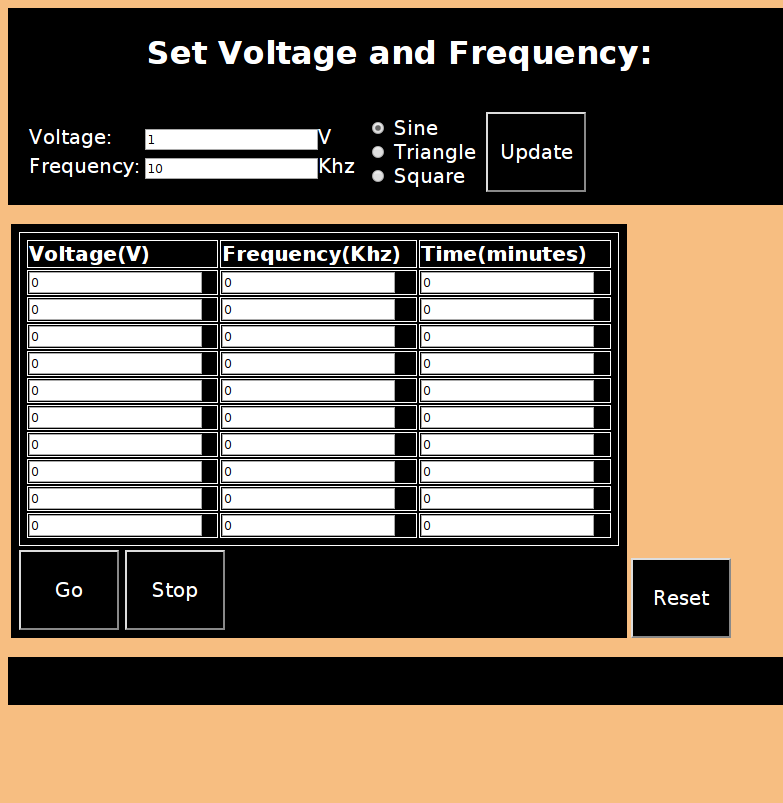
\includegraphics[width=1.0\textwidth,keepaspectratio]{491_web_interface_good.png}
\end{center}
\caption{Web Interface}
\end{figure}

\begin{figure}[!hbt]
\begin{center}
\includegraphics[width=1.0\textwidth,keepaspectratio]{"Diagram - Pi to Minigen and MCP4131"}
\end{center}
\caption{Raspberry Pi Connection Scheme}
\end{figure}

\begin{figure}[!hbt]
\begin{center}
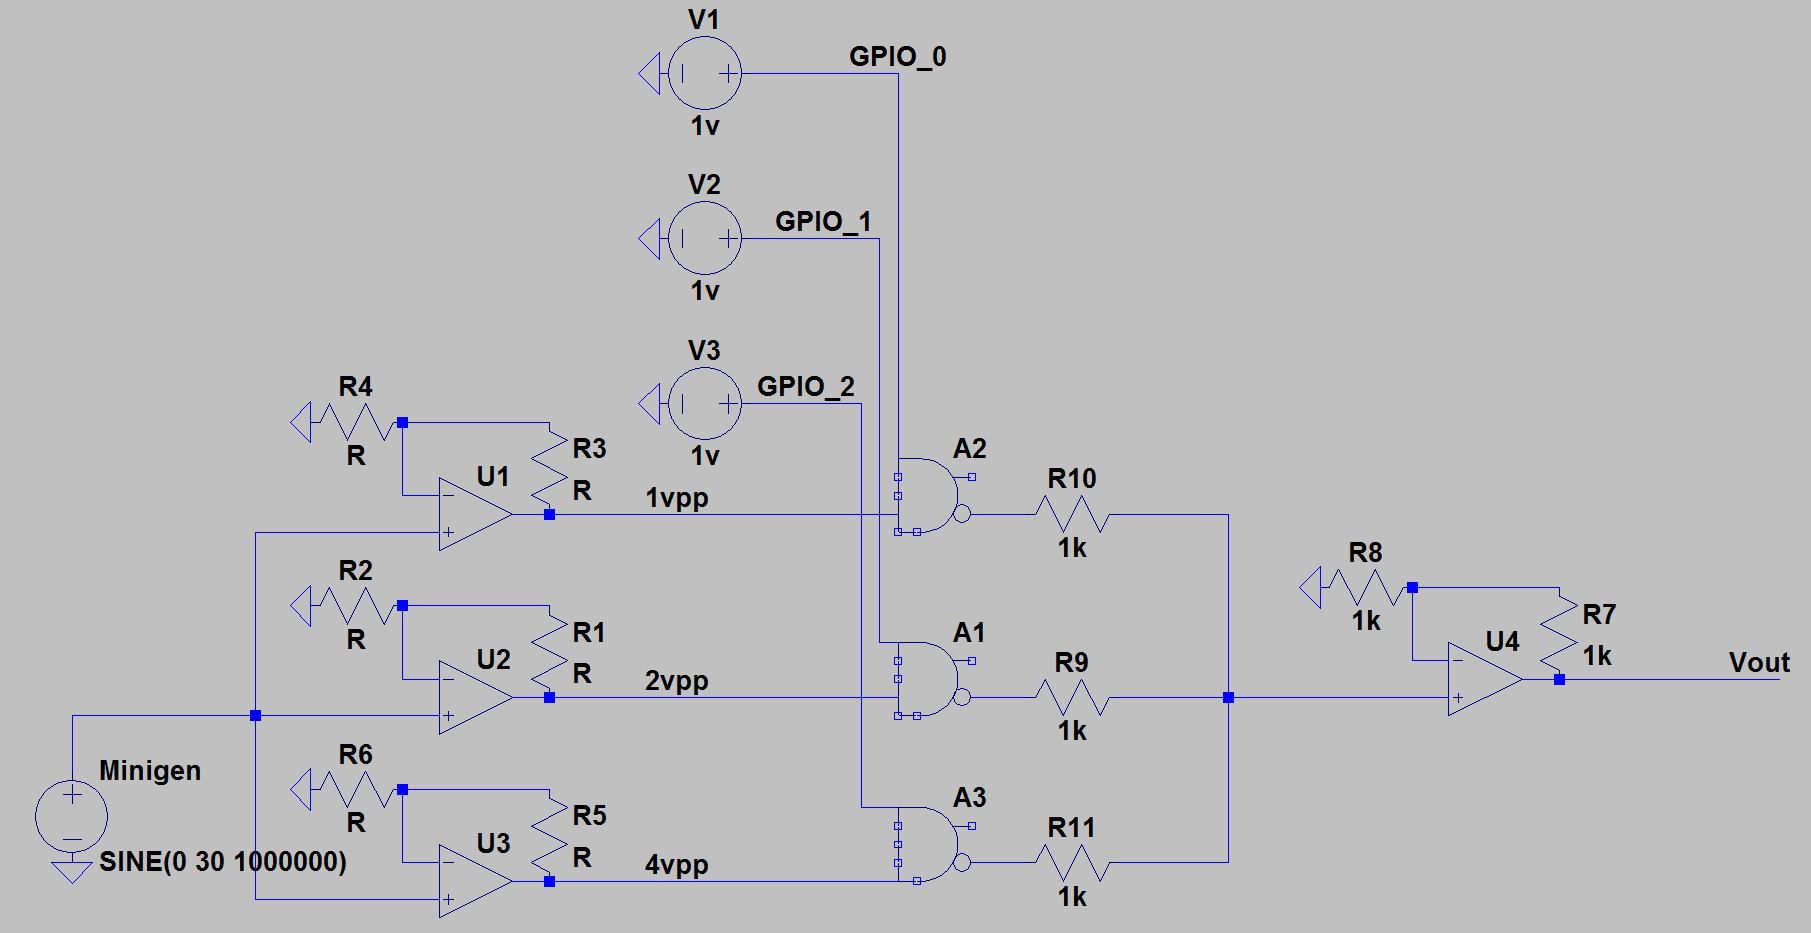
\includegraphics[width=1.0\textwidth,keepaspectratio]{voltage_control_circuit.png}
\end{center}
\caption{Voltage Control Circuit}
\end{figure}

\subsection{Code Listing - HTML}
\lstinputlisting[caption=Main HTML Page]{../www/index.html}

\subsection{Code Listing - CGI Scripts}
% use listinputlisting to list files
\lstinputlisting[caption=Update Website Script]{../cgi-bin/update.py}
\lstinputlisting[caption=Update Voltage and Frequency Script]{../cgi-bin/update_voltage_frequency.py}
\lstinputlisting[caption=Voltage Control Script]{../cgi-bin/voltageControl.py}
\lstinputlisting[caption=Voltage Control Script]{../cgi-bin/voltage_regulator.py}
\lstinputlisting[caption=Minigen Control Script]{../cgi-bin/minigen.py}
\lstinputlisting[caption=PGA Control Script]{../cgi-bin/pga.py}
\lstinputlisting[caption=Reset Script]{../cgi-bin/reset.py}

%\bibliographystyle{unsrt}	% Order by citation
%\bibliography{report}

\end{document}


